% Basic part: charts A1, B1, C1/C2, D1, E1/E2 and the summary table F.
% Every number is a \res... macro from results/basic.tex.

\begin{frame}[b]
  \frametitle{Cena PKO BP rosła przez prawie cały badany okres}
  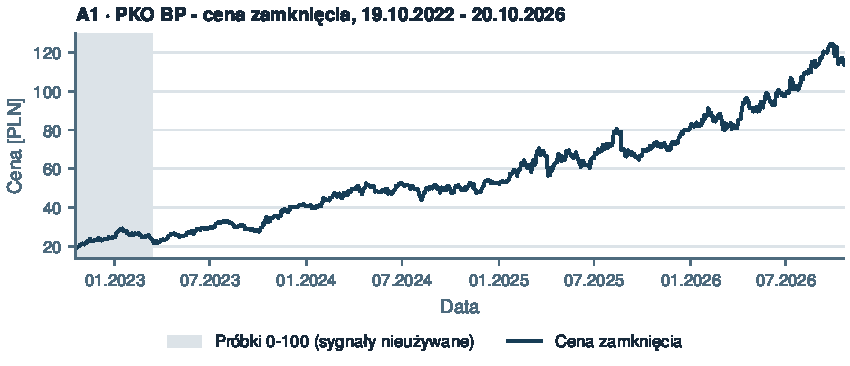
\includegraphics{A1.pdf}\par
  \vskip1mm
  Dane: \resSampleCount{} sesji od \resDataStartDate{} do \resDataEndDate{},
  ceny zamknięcia skorygowane wstecznie (stooq.pl), w PLN. Próbki od 0 do 100
  to tylko rozbieg średnich.
\end{frame}

\begin{frame}[b]
  \frametitle{MACD jest przeważnie dodatni, a jego skala rośnie razem z ceną}
  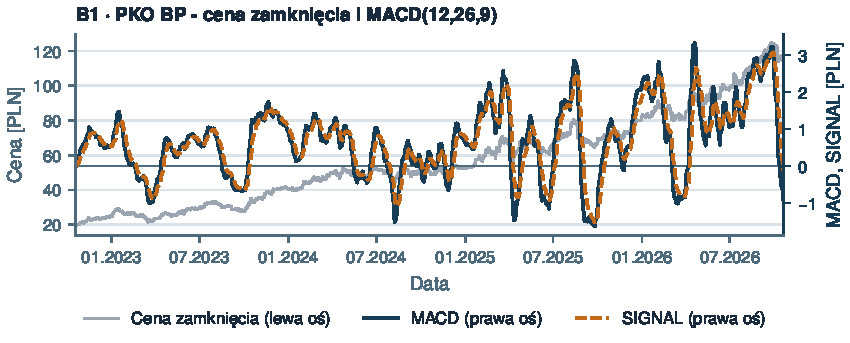
\includegraphics{B1.pdf}\par
  \vskip1mm
  MACD to różnica dwóch EMA w PLN, więc jego skala zależy od ceny, a znak od
  trendu. Przecięcia ceny z liniami MACD nic nie znaczą.
\end{frame}

\begin{frame}[b]
  \frametitle{Malejące słupki histogramu zapowiadają przecięcie i sygnał}
  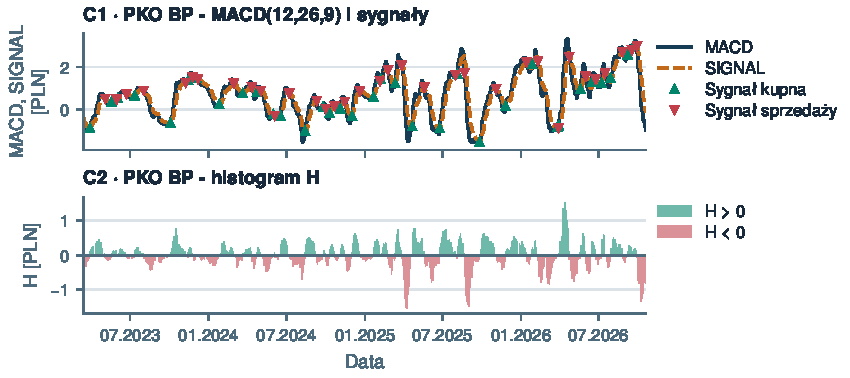
\includegraphics{C1_C2.pdf}\par
  \resSignalCount{} sygnałów od próbki 101, słupki to odległość MACD od SIGNAL.
\end{frame}

\begin{frame}[b]
  \frametitle{Najlepsza transakcja dała \resTradeReturnPct{}\,\% w ciągu
    \resTradeSessions{} sesji}
  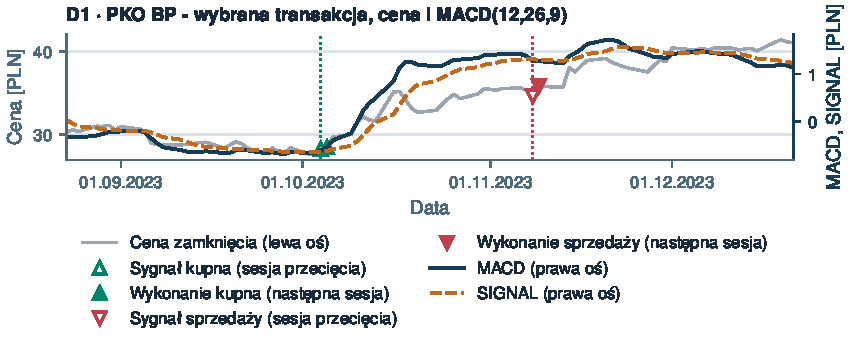
\includegraphics{D1.pdf}\par
  \vskip1mm
  Kupno \resTradeBuyDate{} po \resTradeBuyPrice{} zł, sprzedaż
  \resTradeSellDate{} po \resTradeSellPrice{} zł. MACD przeciął SIGNAL od dołu
  po spadkach i od góry, gdy wzrost wygasł.
\end{frame}

\begin{frame}[b]
  \frametitle{Strategia MACD dała \resReturnPct{}\,\%, a trzymanie akcji
    \resBuyHoldReturnPct{}\,\%}
  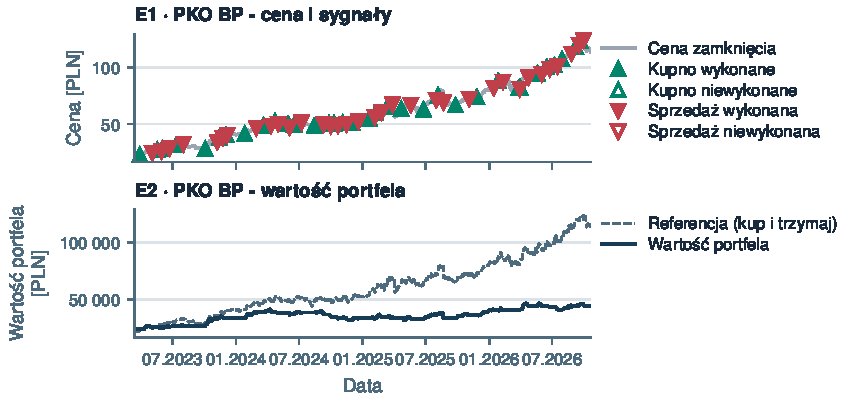
\includegraphics{E1_E2.pdf}\par
  Wykonano \resExecutedSignalCount{} z \resSignalCount{} sygnałów, pozycja otwarta przez
  \resTimeInMarketPct{}\,\% sesji.
\end{frame}

\begin{frame}
  \frametitle{Na PKO BP strategia MACD zarobiła, ale ominęła większość wzrostu,
    bo była w rynku przez \resTimeInMarketPct{}\,\% sesji}
  \renewcommand{\arraystretch}{1.2}
  \begin{tabular*}{\textwidth}{@{}l@{\extracolsep{\fill}}rl@{\hspace{6mm}}r@{}}
    \toprule
    Wielkość & Wartość & Wielkość & Wartość \\
    \midrule
    Kapitał początkowy & \resInitialCapital{} zł
      & Transakcje stratne & \resLosingCount{} z \resClosedCount{} \\
    Wartość końcowa & \resFinalEquity{} zł
      & Skuteczność & \resWinRatePct{}\,\% \\
    Zysk & \resProfitAmount{} zł
      & Największa strata & \resMaxLossPct{}\,\% \\
    Stopa zwrotu R & \resReturnPct{}\,\%
      & Największy zysk & \resMaxGainPct{}\,\% \\
    Transakcje zyskowne & \resProfitableCount{} z \resClosedCount{}
      & Wartość otwartej pozycji & \resOpenValue \\
    Kup i trzymaj & \resBuyHoldReturnPct{}\,\%
      & Czas w rynku & \resTimeInMarketPct{}\,\% \\
    \bottomrule
  \end{tabular*}
  \vskip3mm
  Zyskowne transakcje trwały średnio \resMeanWinSessions{} sesji
  (\resMeanWinPct{}\,\%), stratne \resMeanLossSessions{}
  (\resMeanLossPct{}\,\%). Wniosek dotyczy jednego instrumentu w jednym
  okresie.
\end{frame}
